\chapter{Optomechanical quantum information processing}
\label{ch:Stannigel2012}
% From \cite{Stannigel2012}
%%%%%%%%%%%%%%%%%%%%%%%%%%%%%%%%%%%%%%%%%%%%%%%% 

\section{Introduction}

Optomechanics describes the radiation pressure interaction between an optical
cavity mode and the motion of a macroscopic mechanical object, as it appears,
for example, in a Fabry-P\'{e}rot cavity with a moveable
mirror~\cite{OptoReview}.
First demonstrations of optomechanical (OM)  laser
cooling~\cite{FirstCavityCoolingExp} have recently attracted significant
interest and led to tremendous progress in the development of new fabrication
methods and experimental techniques for controlling OM interactions at the
quantum level.
Apart from ground-state cooling~\cite{TeufelNature2011,ChanNature2011}, this
includes the demonstration of slow
light~\cite{WeisScience2010,SafaviNaeiniNature2011}, and the coherent
interconversion of optical and mechanical
excitations~\cite{FiorePRL2011,VerhagenNature2012}. These achievements pave the
way for a new type of quantum light-matter interface and give rise to
interesting perspectives for novel OM-based quantum technologies. As a
solid-state approach, such an all-OM platform would benefit directly from
advanced nanofabrication and scalable integrated photonic circuit techniques. At
the same time, long mechanical lifetimes comparable to those of atomic systems
allow us to combine optical nonlinearities with a stationary quantum memory for
light.

In this work we study strong OM coupling effects in \emph{multimode} OM systems
(OMSs) and describe how resonant or near-resonant interactions in this setting
allow us to exploit the intrinsic nonlinearity of radiation pressure in an
optimal way. Our approach is based on the resonant exchange of photons between
two optical modes mediated by a single phonon. This resonance induces much
stronger nonlinearities than achievable in single-mode OMSs, where nonlinear
effects  are suppressed by a large mechanical
frequency~\cite{MarshallPRL2003,LudwigNJP2008,RablPRL2011,NunnenkampPRL2011}.
Consequently, multimode OMSs provide a promising route for accessing the
single-photon strong-coupling regime, where the coupling $g_0$ as well as the
mechanical frequency $\omega_m$ exceeds the cavity decay rate
$\kappa$~\cite{RablPRL2011}.
This regime is within reach of state-of-the-art nanoscale OM
devices~\cite{ChanNature2011,EichenfieldNature2009,CarmonPRL2007,DingAPL2011} or
analogous cold atom OMSs~\cite{GuptaPRL2007,BrenneckeScience2008}, and here we
discuss how strong OM interactions in a multimode setup can be used to generate
single photons and to perform controlled gate operations between photonic or
mechanical qubits.
Combined with very recently developed photon-phonon interfaces and quantum
memories based on linearized OM couplings~\cite{FiorePRL2011,VerhagenNature2012,
Painter2011}, our results provide a basis for efficient OM classical and quantum
information processing with applications ranging from photon transistors to
quantum repeaters and networks.
\begin{figure}
\begin{center}
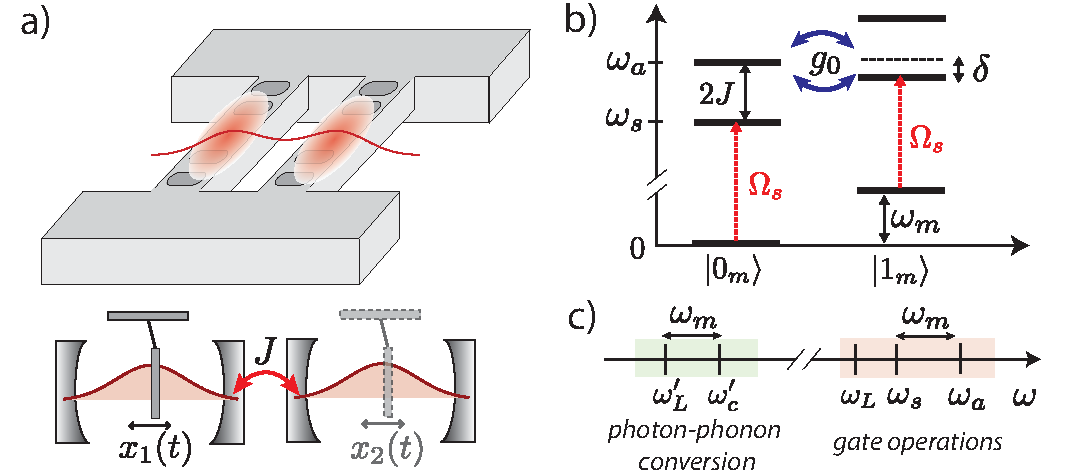
\includegraphics[width=0.9\textwidth]{./figs_Stannigel2012/Figure1.pdf}
\caption
[Model of two resonators]
{ a) Setup of two tunnel-coupled OM crystal cavities (see
Ref.~\cite{EichenfieldNature2009,ChanNature2011} for more details).  b) Level
diagram showing the lowest mechanical and optical excitations in a two mode OMS.
Resonant coupling $(\delta=0)$ occurs when the tunnel splitting $2J$ between the
optical modes is comparable to the mechanical frequency $\omega_m$. c) Different
sets of strongly and weakly coupled optical modes and control laser fields can
be used for nonlinear interactions $(\omega_{s},\omega_{a},\omega_L)$ and purely
linear photon storage and retrieval operations
$(\omega_c^\prime,\omega_L^\prime)$.
}
\label{fig:Setup}
\end{center} 
\end{figure}


\section{Model} 

We consider a setup of two tunnel-coupled
OMSs~\cite{MiaoPRL2009,GrudininPRL2010,DobrindtPRL2010,Painter2011,CheungPRA2011}
as schematically shown in Fig.~\ref{fig:Setup}, focusing on the OM crystal
design~\cite{EichenfieldNature2009,ChanNature2011} as a specific example.
Each OMS $i=1,2$ is represented by an optical mode of frequency $\omega_c$ and a
bosonic operator $c_{i}$, which is coupled via optical gradient forces to the
motion of an isolated mechanical mode $b_i$ with vibrational frequency
$\omega^i_m$.  The Hamiltonian for this system is $(\hbar=1)$
\begin{equation}\label{eq:H}
\begin{split}
H= &\sum_{i=1,2} \omega_m^i b_i^\dag b_i +  \omega_c c_i^\dag c_i + g_0 c_i^\dag
c_i (b_i+ b_i^\dag) \\
&- J (c_1^\dag c_{2} + c_{1} c_{2}^\dag) +   \sum_{i=1,2}  \Omega_i ( c_i 
e^{i\omega_L t} + �{\rm H.c.}),
\end{split}\end{equation}
where $J$ is the tunneling amplitude between the optical modes and $g_0$ denotes the single-photon OM coupling; $\Omega_i$ are the local amplitudes of external control laser fields of frequency $\omega_L$.  Below we also consider an additional set of cavity modes and driving fields with frequencies $\omega_c^\prime $ and  $\omega_L^\prime$, respectively.  
As indicated in Fig.~\ref{fig:Setup}(c), we assume these modes to be separated in frequency and used for cooling the mechanical modes~\cite{WilsonRaePRL2007,MarquardtPRL2007}, and linear photon storage and retrieval operations~\cite{FiorePRL2011,VerhagenNature2012,ZhangPRA2003,AkramNJP2010} only.

Apart from the coherent dynamics described by Eq.~\eqref{eq:H}, we include
dissipation through cavity decay and mechanical damping and model the evolution
of the system density operator $\rho$ by a master equation (ME)
\begin{equation}\label{eq:ME}
\begin{split}
\dot \rho = &-i[H,\rho] + \sum_{i}  \kappa \mathcal{D}[c_i] \rho +
\mathcal{L}_\gamma \rho, \\
\end{split} 
\end{equation}
where  $\mathcal{D}[c]\rho=2c\rho c^\dag-\{c^\dag c, \rho\}_+ $, and
$\mathcal{L}_\gamma =\sum_i \frac{\gamma}{2}  (N_{\rm th}+1)   \mathcal{D}[b_i]
+ \frac{\gamma}{2}  N_{\rm th}  \mathcal{D}[b_i^\dag]$.
Here,  $\kappa$ is the optical field decay rate, $\gamma=\omega_m/Q$ the
mechanical damping rate for a quality factor $Q$ and $N_{\rm th}=(e^{\hbar
\omega_m/k_BT}-1)^{-1}$ the mechanical equilibrium occupation number for
temperature $T$. Below we identify $\Gamma_m=\frac{\gamma}{2}(3N_{\rm
th}+\frac{1}{2})$ as the characteristic decoherence rate for mechanical qubit
states~\cite{DecoherenceRate}.
\begin{figure}
\begin{center}
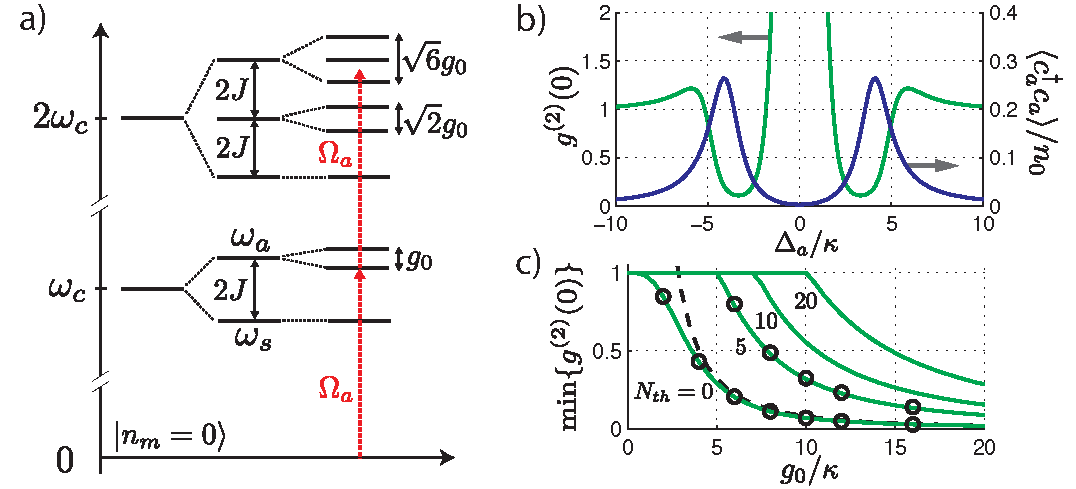
\includegraphics[width=1\textwidth]{./figs_Stannigel2012/Figure2.pdf}
\caption
[Behavior of the coupled system]
{a) Energy level diagram of a resonantly coupled OMS,
$\delta=2J-\omega_m=0$, and for a single mechanical mode in the ground state. b)
Excitation spectrum and $g^{(2)}(0)$ for a weak coherent field exciting the
$c_a$ mode, where $g_0/\kappa=8$ and $n_0=\Omega^2_a/\kappa^2$.  c) Minimal
value of $g^{(2)}(0)$  as a function of the OM coupling strength $g_0$ and for
different values of $N_{\rm th}$. The analytical results (solid lines) given in
the text are in good agreement with exact numerics (circles). The dashed line
shows the asymptotic scaling $\sim 8\kappa^2/g_0^2$ at zero temperature.}
\label{fig:ResonantLevels}
\end{center} 
\end{figure}



\section{Resonant strong-coupling optomechanics}
 
We focus on the strong coupling regime $\omega_m,g_0\gg \kappa,\Gamma_m$,  and
our main goal is to show how the multimode OMS described by Eq.~\eqref{eq:H} can
be used for implementing controlled interactions between qubits encoded in
photonic or phononic degrees of freedom.  To illustrate this we first consider a
single mechanical resonator, $b\equiv b_1$, $\omega_m\equiv \omega_m^1$. We
introduce symmetric and antisymmetric optical modes $c_{s,a}=  \left( c_1 \pm
c_2\right)/\sqrt{2}$ with eigenfrequencies $\omega_{s,a}$ split by $2J$.
Further, we assume that $\omega_m\sim 2J \gg g_0,\kappa, |\delta|$, where
$\delta=2J-\omega_m$  (see Fig.~\ref{fig:Setup}(b)). This condition can be
achieved in nanoscale OMSs where $\omega_m\sim $
GHz~\cite{EichenfieldNature2009,ChanNature2011,CarmonPRL2007,DingAPL2011} and a
matching tunnel splitting can be designed by appropriately adjusting the spacing
between the cavities~\cite{EichenfieldNature2009,GrudininPRL2010}. In this
regime we can make a rotating wave approximation with respect to the large
frequency scale $\omega_m \sim 2J$ and after changing into a frame rotating with
$\omega_L$ we obtain~\cite{GrudininPRL2010}
\begin{equation}\label{eq:HRWA}
H= - \Delta_s c_s^\dag c_s - \Delta_a  c_a^\dag c_a   + \omega_m b^\dag b 
+ \frac{g_0}{2} (c_a c_s^\dag b^\dag +    c_a^\dag c_s  b)+ H_\Omega(t).
\end{equation}
Here $ \Delta_{s,a}= \omega_L - \omega_{s,a}$ are the detunings of the driving
field from the $c_s$ and $c_a$ mode, respectively, and
$H_\Omega(t)=\sum_{\eta=s,a} \left(\Omega_\eta(t) c_\eta + {\rm H.c.}\right)$
accounts for the external driving fields with slowly varying amplitudes
$\Omega_{s,a}(t)=(\Omega_1(t)\pm\Omega_2(t))/\sqrt{2}$.

The two-mode OM coupling in Eq.~\eqref{eq:HRWA} describes  photon transitions
between the energetically higher mode $c_a$ to the lower mode $c_s$, while
simultaneously absorbing or emitting a phonon.  For
$(\Delta_s-\Delta_a-\omega_m)=\delta=0$, this leads to a resonant interaction
between states $|n_a,n_s,n_m\rangle$ and $|n_a-1,n_s+1,n_m+1\rangle$, where
$n_a$, $n_s$ and $n_m$ label the occupation numbers of the two optical modes and
the mechanical mode, respectively.  In analogy to atomic cavity quantum
electrodynamics (QED)~\cite{CavityQEDReview}, the nonlinear scaling of the
corresponding transition amplitudes $\frac{g_0}{2} \sqrt{n_a (n_s+1) (n_m+1)}$
results in an anharmonic level diagram as shown in
Fig.~\ref{fig:ResonantLevels}(a).  If $g_0$ exceeds the cavity linewidth
$\kappa$, one and two photon transitions can be spectrally resolved, indicating
the onset of strong single-photon nonlinearities.


\section{An OM single-photon source}
 
As a potential first application of the nonlinear OM interaction we discuss the
use of the OMS as a single-photon source, which is characterized by a vanishing
equal time two-photon correlation function $g^{(2)}(0)$.  In
Fig.~\ref{fig:ResonantLevels}(b) we plot the excitation spectrum $\langle
c_a^\dag c_a \rangle$ and $g^{(2)}(0)=\langle c_a^\dag c_a^\dag c_a
c_a\rangle/\langle c_a^\dag c_a\rangle^2$,  for the case where only the $c_a$
mode is weakly driven. Around the single-photon resonances $\Delta_a=\pm g_0/2$
we observe strong anti-bunching $g^{(2)}(0)<1$ as a clear signature of
non-classical  photon statistics. To quantify this effect we assume that
$\Gamma_m \ll\kappa$, which allows us to treat subspaces connected to different
$|n_m\rangle$ separately.  For weak driving fields $\Omega_a\ll\kappa$, the
system dynamics can then be restricted to the  six states $ |0_a,0_s,
n_m\rangle, |1_a,0_s, n_m\rangle,|0_a,1_s, n_m+1\rangle,|2_a,0_s, n_m\rangle,
|1_a,1_s, n_m+1\rangle,|0_a,2_s, n_m+2\rangle$ and  we calculate the relevant
occupation probabilities $p_{1,0,n_m}$ and  $p_{2,0,n_m}$ to leading order in
$\Omega_a$~\cite{Carmichael1991}.
We obtain
\begin{equation}
p_{1,0,n}=\abs{ \frac{4\Omega_a d}{ X_n}}^2, \qquad p_{2,0,n} = 8 \abs{
\frac{\Omega_a^2 (8 d^2 - g_0^2)}{( X_n (2X_n -g_0^2))}}^2,
\end{equation}
where $d = \Delta_a - i\kappa$ and $X_n=d^2-g_0^2(n+1)$. By taking the
appropriate thermal averages, $\ev{n_a} = \sum_n \zeta_n p_{1,0,n}$ and
$g^{(2)}(0)  = 2 \sum_n \zeta_n p_{2,0,n}/\ev{n_a}^2$, where
$\zeta_n=(1-e^{-\beta \hbar \omega_m})e^{-\beta \hbar \omega_m n}$ and
$\beta^{-1}=k_B T$, the two photon correlation function can be evaluated for
arbitrary temperatures $T$.

In Fig.~\ref{fig:ResonantLevels}(c) we plot the minimal value of $g^{(2)}(0)$ as
a function of the coupling strength $g_0$ and for different $N_{\rm th}$.
As the OM coupling increases we find that for $T=0$ the minimum of the
correlation function scales as $\textrm{min}_{\Delta_a}\{g^{(2)}(0)\}\simeq 8
\kappa^2/g_0^2$. This demonstrates an improved scaling over off-resonant photon
blockade effects in single-mode OMSs, where for large $\omega_m$ only a small
reduction $g^{(2)}(0)\simeq 1-g_0^2 /(\kappa \omega_m)$ can be
obtained~\cite{RablPRL2011}. Since the positions of the single and two-photon
resonances depend explicitly on the mechanical state $|n_m\rangle$,  finite
temperature degrades the quality of the single-photon source.  Nevertheless,
with increasing coupling strength the anti-bunching effect becomes surprisingly
robust and when combined with cooling cycles to achieve $\langle n_m\rangle \sim
1$~\cite{ChanNature2011}, allows the operation of OM single-photon sources even
at environmental temperatures of a few Kelvin.
\begin{figure}
\begin{center}
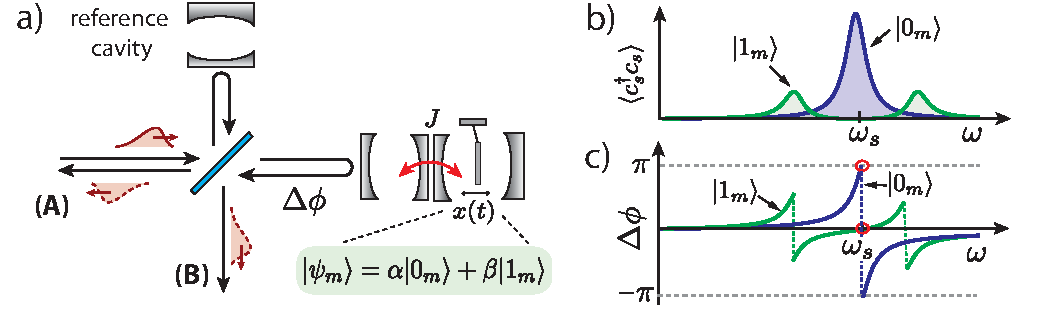
\includegraphics[width=1\textwidth]{./figs_Stannigel2012/Figure3.pdf}
\caption
[A single-phonon single-photon transistor]
{a) An incoming
photon in port (A) passes through the interferometric setup and leaves through
port (A) or (B), depending on the phase shift $\Delta \phi$ acquired upon
reflection from the two-mode OMS.   b), c) For a mechanical system in state
$|0_m\rangle$, the OMS exhibits a single resonance at $\omega_s$ $(\Delta
\phi=\pi$), while for state $|1_m\rangle$  the resonance splits by $g_0\gg
\kappa $ and the photon does not enter the cavity $(\Delta \phi=0)$.  }
\label{fig:SinglePhononTransistor}
\end{center} 
\end{figure}

\section{Single-phonon single-photon transistor}  
Given the ability to generate single photons,
Fig.~\ref{fig:SinglePhononTransistor} illustrates a basic scheme for using the
same resonant OMS to implement a two-qubit gate~\cite{DuanPRL2004}. First, we
assume that the state of a control photon is mapped onto a mechanical
superposition state  $\alpha|0_m\rangle+\beta |1_m\rangle$.
This can be achieved with conventional cooling followed by photon-phonon
conversion techniques using linearized OM interactions with an auxiliary mode
$\omega_c^\prime$ (see Fig.~\ref{fig:Setup}(c)). Next, a single target photon of
central frequency $\sim \omega_s$ is sent through the interferometric setup as
described in Fig.~\ref{fig:SinglePhononTransistor}.
If the mechanical mode is in the state $|0_m\rangle$,  the incoming photon
couples to a single resonant state $|0_a,1_s,0_m\rangle$ (see
Fig.~\ref{fig:Setup}(b)), such that it enters the cavity and picks up a phase
before being reflected.  Instead, if the mechanical resonator is in the state 
$|1_m\rangle$,  the resonant coupling between $|0_a,1_s,1_m\rangle$ and
$|1_a,0_s,0_m\rangle$ splits the cavity resonance, and for $g_0>\kappa$ the
photon is reflected without a phase shift.
Under ideal conditions,  the final result is an entangled state
\begin{equation}\label{eq:Entangled}
|\psi\rangle = \alpha | 0_m, 1_A,0_B\rangle + \beta | 1_m, 0_A,1_B\rangle,
\end{equation}
where $A$ and $B$ are the two ports of the interferometer. This state can be
converted back into an entangled state between the initial control and target
photon.

Assuming that the storage and retrieval of the control photon can be achieved
with high fidelity, the error for producing the entangled
state~\eqref{eq:Entangled} with $\alpha=\beta=1/\sqrt{2}$ is approximately given
by
\begin{equation}\label{eq:Error}
\epsilon  \approx  \frac{4\kappa^2}{g_0^2}+  \frac{1}{(\tau_p \kappa)^{2}}+ 
\tau_p \Gamma_m,
\end{equation} 
where  $\tau_p$ is the duration of the single-photon pulse. The individual
contributions in Eq.~\eqref{eq:Error} arise from an imperfect photon reflection,
the finite spectral width of the photon pulse, and mechanical decoherence,
respectively.
A minimal error is achieved for  $\tau_p^{-1}\approx \sqrt[3]{\kappa^2
\Gamma_m}$ where we obtain $\epsilon\approx {\rm  max} \{  4\kappa^2/g_0^2,
\sqrt[3]{\Gamma_m^2 /\kappa^2}\}$.
Assuming an OM crystal device with $\omega_m/(2\pi)=4$ GHz and $Q=10^5$ as
discussed in Ref.~\cite{ChanNature2011}, but with an improved OM coupling
$g_0/(2\pi)=50$ MHz and a lower  decay rate $\kappa/(2\pi)=5$ MHz, we obtain
gate errors $\epsilon\approx 0.1$ for environmental temperatures around
$T\approx 100$ mK.




\section{Phonon-phonon interactions}
  
Finally, we consider the possibility to perform a 
controlled gate operation between two qubits stored
in long-lived mechanical modes.
Our approach is depicted 
in Fig.~\ref{fig:PhononQuantumGate}(a), 
and combines the long coherence times of an OM 
quantum memory~\cite{FiorePRL2011,VerhagenNature2012,ZhangPRA2003,AkramNJP2010} 
with the practical utility of exploiting interactions 
between stationary phononic qubits.
We focus on the limit $\Gamma_m\ll \kappa$, 
and assume that optical (e.g. `path encoded') 
qubits are first mapped onto long-lived states $|0_m\rangle$ 
and $|1_m\rangle$ of two or more mechanical modes.
The OM coupling is then employed to generate 
nonlinear interactions between the phonons only.  
\begin{figure}
\begin{center}
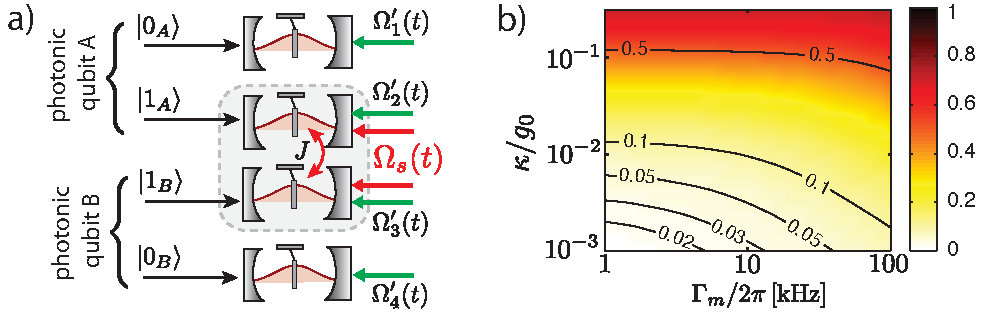
\includegraphics[width=1\textwidth]{./figs_Stannigel2012/Figure4.pdf}
\caption
[Controlled phase gate]
{a) OM quantum memory, where `path-encoded' photonic
qubits are stored in long-lived mechanical states using tunable linearized OM
interactions $\sim\Omega^\prime_i(t)$. Deterministic gate operation between
stationary qubits are implemented by a controlled phonon-phonon interaction
$\sim\Omega_s(t)$ as described in the text. b) The total error $\epsilon_g$ for
implementing a controlled phase gate between two phononic qubits is minimized
with respect to $\Delta_s$ and plotted as a function of $\kappa$ and $\Gamma_m$
(see text). The parameters for this plot are $g_0/(2\pi)=50$ MHz,
$\gamma/(2\pi)=4$ kHz, $\alpha=1$ and $g_0/\delta=1/3$.
}
\label{fig:PhononQuantumGate}
\end{center} 
\end{figure}


We consider nonlinear interactions between
two mechanical modes $b_1$ and $b_2$ described
by Eq.~\eqref{eq:H}, detuned from resonance such that
$g_0< |(2J-\omega_m^i)|$ and direct transitions between  
photons and phonons are suppressed. 
To obtain the effective phonon-phonon interactions,
we first diagonalize
$H$ to second order in $\xi_i = g_0/(2J-\omega_m^i)$
with the transformation
$H\rightarrow e^{iS}He^{-iS}$, 
where 
$S=\frac{i}{2} (c_s^\dag c_a (\xi_1b_1^\dag-\xi_2b_2^\dag) -{\rm H.c.})$.
This yields
 $H= H_0 +H_g+H_\Omega(t)$, where $H_0=  - \Delta_s c_s^\dag c_s - \Delta_a 
 c_a^\dag c_a   + \sum_i \omega^i_m b_i^\dag b_i$,
\begin{equation}\label{eq:Hoff}
	H_g= \frac{g_0}{4} \left[ (c_s^\dag c_s\!+\!1)c^\dag_a c_a (\xi_1\!+\!\xi_2) 
	+ (c_a^\dag c_a\! -\!	c_s^\dag c_s) \mathcal{N}_b \right],
\end{equation}
and we have neglected small corrections to the driving Hamiltonian
$H_\Omega(t)$.
The phonon operator in Eq.~\eqref{eq:Hoff} is given by $\mathcal{N}_b= \xi_1
b_1^\dag b_1+\xi_2 b_2^\dag b_2 - (\xi_1+\xi_2)(b_1^\dag b_2+ b_2^\dag b_1)/2$.
For simplicity we focus on symmetric detuning, $\omega_m^{1,2} = 2J\mp \delta$,
where $\mathcal{N}_b=\frac{g_0}{\delta}(b_1^\dag b_1-b_2^\dag b_2)$.
The  transformation also modifies the dissipative terms in the
Eq.~\eqref{eq:ME}; most importantly, we find an optically-induced decay channel
for the mechanical modes, $\mathcal{L}_\gamma\rightarrow \mathcal{L}_\gamma +
\kappa g^2_0/(4\delta^2) \mathcal{D}[c_s (b_1+b_2)]$.

We assume that only the $c_s$ mode is weakly 
driven by a slowly-varying control field $\Omega_s(t)$. 
In this case the $c_a$ mode remains unpopulated and 
we neglect it. 
Next, we shift the driven mode, $c_s\rightarrow \alpha + c_s$, 
by the classical amplitude $\alpha$,
yielding an effective ME  for $c_s$, $b_1$ and $b_2$.
Finally, we adiabatically eliminate the $c_s$ mode, valid in the
limit $|\alpha|\sim \mathcal{O}(1)$ and $(g_0^2|\alpha|/4\delta)\ll
|\Delta_s+i\kappa|$,
to obtain an effective ME for the mechanical modes~\cite{SM},
\begin{equation}\label{eq:Effective}
\begin{split}
\dot \rho_m =& -i[H_m + \Lambda (b_1^\dag b_1-b_2^\dag b_2)^2 �, \rho_m ] 
+\mathcal{L}_\gamma \rho_m\\
&+ \Gamma_\phi \mathcal{D}[(b_1^\dag b_1-b_2^\dag b_2)]\rho_m   + 
\frac{\gamma^\prime}{2} \sum_i   \mathcal{D}[b_i]\rho_m.
\end{split} 
\end{equation}
Here, $\gamma^\prime=\kappa |\alpha|^2 g_0^2/(2\delta^2)$, and the phonon-phonon
interaction and the phonon dephasing rate are given by
\begin{equation}
\Lambda=\frac{g_{0}^{4}|\alpha|^2  \Delta_{s}}{16 \delta^2
(\Delta_{s}^{2}+\kappa^{2})},\qquad \Gamma_\phi= \frac{g_{0}^{4}|\alpha|^2 
\kappa}{16\delta^2(\Delta_{s}^{2}+\kappa^{2})}.
\end{equation}
The effective Hamiltonian in Eq.~\eqref{eq:Effective} describes 
a phonon nonlinearity with a tunable strength $\Lambda(t)\sim |\alpha(t)|^2$. 
The relevant cross-coupling is given by 
\begin{equation}\label{eq:Heff}
H_{\rm int} \simeq 2 \Lambda b_1^\dag b_1  b_2^\dag b_2,
\end{equation}
and when acting for a time $t_g=\pi/(2\Lambda)$, this Hamiltonian implements a
controlled-phase gate between two qubits encoded in states $|0_m\rangle$ and
$|1_m\rangle$.
During this time, phonons experience intrinsic and optically-induced decoherence
as seen in Eq.~\eqref{eq:Effective}.
In Fig.~\ref{fig:PhononQuantumGate}, we plot the
resulting gate error $\epsilon_g=1-\langle\psi_0|\rho_m(t_g)|\psi_0\rangle$  
for an initial state
$|\psi_0\rangle=\frac{1}{2}(|0_m\rangle+|1_m\rangle)^{\otimes2}$
optimized with respect to $\Delta_s$.
Using the total decoherence rate of this state, 
$\Gamma_{\rm decoh}= 2\Gamma_m+ \Gamma_\phi+ \gamma^\prime/2$, 
we find that  $\epsilon_g\propto\Gamma_{\rm decoh}/\Lambda$ 
is minimized for $|\Delta_s|\simeq g_0/2$, where $\epsilon_g\propto
4(\kappa/g_0)$.
While this scaling with $g_0$ is weaker than for a gate based on photon
reflection (see Eq.~\eqref{eq:Error}), the ability to perform a gate between
stationary qubits represents an important advantage of this approach.

 
\section{Conclusions} 

We have described single-photon and single-phonon nonlinear effects in strongly
coupled multimode OMSs. We have shown how induced nonlinearities on or near
resonance can be used for controlled quantum gate operations between flying
optical or stationary phononic qubits. Our results provide a realistic route
towards the quantum nonlinear regime of OMSs, and a framework for future OM
information processing applications.
